\documentclass[border=10pt]{standalone}
\usepackage[svgnames]{xcolor}
\usepackage{amsmath}
\usepackage{pgfplots}
\pgfplotsset{compat=newest}
\usepackage[sfdefault]{FiraSans}
\usepackage{FiraMono}
\renewcommand*\familydefault{\sfdefault}
\begin{document}
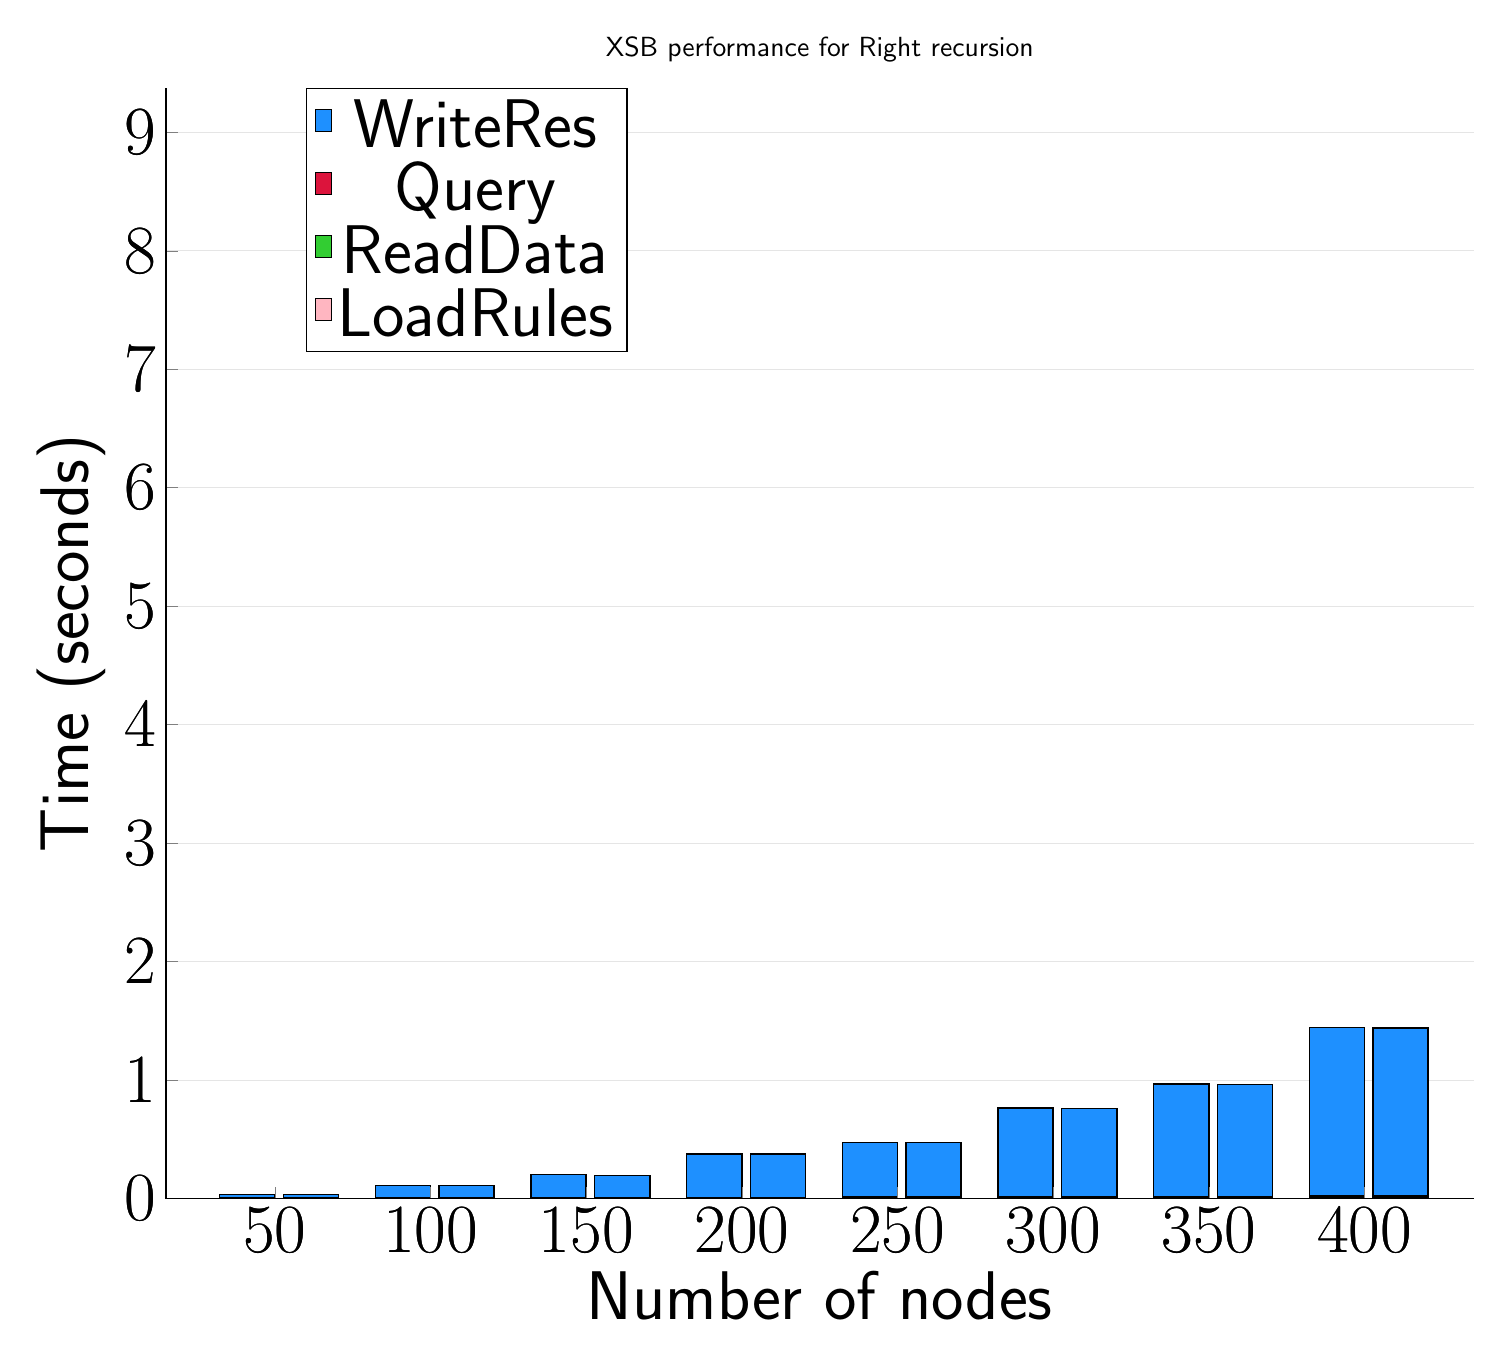
\begin{tikzpicture}
\begin{axis}[
   ybar stacked,
   title={XSB performance for Right recursion},
   bar shift=-10pt,
   width=1.5\textwidth,
   bar width=0.7cm,
   ymajorgrids, tick align=inside,
   major grid style={draw=gray!20},
   xtick=data,
   ymin=0, ymax=9.375487327575684,
   axis x line*=bottom,
   axis y line*=left,
   enlarge x limits=0.1,
   legend style={
       at={(0.23, 1)},
       anchor=north,
       legend columns=1,
       font=\Huge,
   },
   ylabel={Time (seconds)},
   xlabel={Number of nodes},
   label style={font=\Huge},
   tick label style={font=\Huge},
]
\addlegendimage{fill=DodgerBlue, draw=black, line width=0.2pt}
\addlegendentry{WriteRes}
\addlegendimage{fill=Crimson, draw=black, line width=0.2pt}
\addlegendentry{Query}
\addlegendimage{fill=LimeGreen, draw=black, line width=0.2pt}
\addlegendentry{ReadData}
\addlegendimage{fill=LightPink, draw=black, line width=0.2pt}
\addlegendentry{LoadRules}
\addplot +[fill=LightPink, draw=black, line width=0.5pt] coordinates {
    (50, 0.0038324197133382133)
    (100, 0.00400376319885254)
    (150, 0.00358994801839193)
    (200, 0.0033346811930338566)
    (250, 0.0037192503611246735)
    (300, 0.0032596588134765595)
    (350, 0.00319202740987142)
    (400, 0.0035860538482666003)
};
\addplot +[fill=LimeGreen, draw=black, line width=0.5pt] coordinates {
    (50, 0.0018213589986165399)
    (100, 0.0031759738922119128)
    (150, 0.003994703292846677)
    (200, 0.004513661066691084)
    (250, 0.005610386530558269)
    (300, 0.006181955337524417)
    (350, 0.006823619206746421)
    (400, 0.008533318837483721)
};
\addplot +[fill=Crimson, draw=black, line width=0.5pt] coordinates {
    (50, 0.00034562746683756534)
    (100, 0.0012365976969401042)
    (150, 0.00207034746805827)
    (200, 0.0036316712697346963)
    (250, 0.005029916763305663)
    (300, 0.007635037104288737)
    (350, 0.008720080057779947)
    (400, 0.013995329538981102)
};
\addplot +[fill=DodgerBlue, draw=black, line width=0.5pt] coordinates {
    (50, 0.028127590815226238)
    (100, 0.10409967104593892)
    (150, 0.19288929303487143)
    (200, 0.36627427736918133)
    (250, 0.4601223468780517)
    (300, 0.7482695579528805)
    (350, 0.946849902470906)
    (400, 1.4191269874572756)
};
\end{axis}
\begin{axis}[
   ybar stacked,
   bar shift=13pt,
   width=1.5\textwidth,
   bar width=0.7cm,
   ymajorgrids, tick align=inside,
   major grid style={draw=none},
   xtick=data,
   ymin=0, ymax=9.375487327575684,
   axis x line*=none,
   axis y line*=none,
   enlarge x limits=0.1,
   label style={font=\Huge},
   tick label style={font=\Huge},
]
\addplot +[fill=LightPink, draw=black, line width=0.5pt] coordinates {
    (50, 0.0032619999999999997)
    (100, 0.004002999999999997)
    (150, 0.002957333333333333)
    (200, 0.003335)
    (250, 0.0028476666666666667)
    (300, 0.002731666666666667)
    (350, 0.0025189999999999965)
    (400, 0.003548666666666667)
};
\addplot +[fill=LimeGreen, draw=black, line width=0.5pt] coordinates {
    (50, 0.0016506666666666633)
    (100, 0.0031773333333333337)
    (150, 0.003193333333333333)
    (200, 0.004514000000000003)
    (250, 0.005553)
    (300, 0.00616)
    (350, 0.006779333333333329)
    (400, 0.008534666666666668)
};
\addplot +[fill=Crimson, draw=black, line width=0.5pt] coordinates {
    (50, 0.00030633333333333234)
    (100, 0.001236666666666671)
    (150, 0.0016990000000000032)
    (200, 0.0036329999999999995)
    (250, 0.004687333333333333)
    (300, 0.00755733333333333)
    (350, 0.008103)
    (400, 0.013977333333333333)
};
\addplot +[fill=DodgerBlue, draw=black, line width=0.5pt] coordinates {
    (50, 0.028153333333333336)
    (100, 0.10407366666666668)
    (150, 0.18631799999999998)
    (200, 0.363882)
    (250, 0.4597076666666667)
    (300, 0.744996)
    (350, 0.9466123333333334)
    (400, 1.414103)
};
\end{axis}
\end{tikzpicture}

\end{document}
